\begin{frame}
  \frametitle{\textbf{Centrality}}
  \begin{columns}
    \column{0.5\textwidth}
    \begin{itemize}
    \item \textbf{Centrality} is a measure of the nuclear overlap in a collision event
    \item Derived from multiplicity distibutions, forward-energy distribution
    \item Essential for categorizing events based on QGP-formation status
    \item Relate observables back to impact parameter via Glauber model
    \end{itemize}

    \

    \centering
    \begin{tikzpicture}
      \node{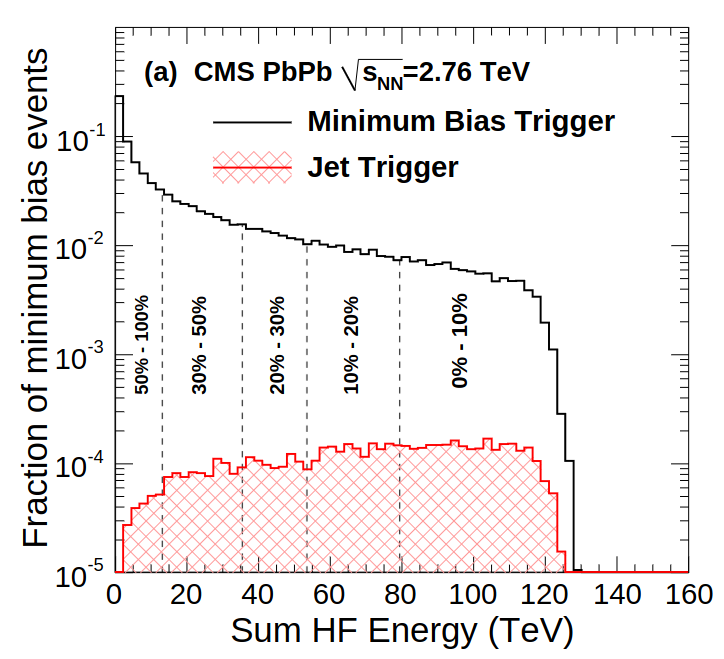
\includegraphics[width=0.7\textwidth]{centrality-hf-energy.png}};
      \node[font=\tiny] at (1.5,-2) {\href{https://arxiv.org/abs/1408.2549}{arXiv:1408.2549}};
    \end{tikzpicture}
    \column{0.5\textwidth}
    \centering
    \begin{tikzpicture}
      \node{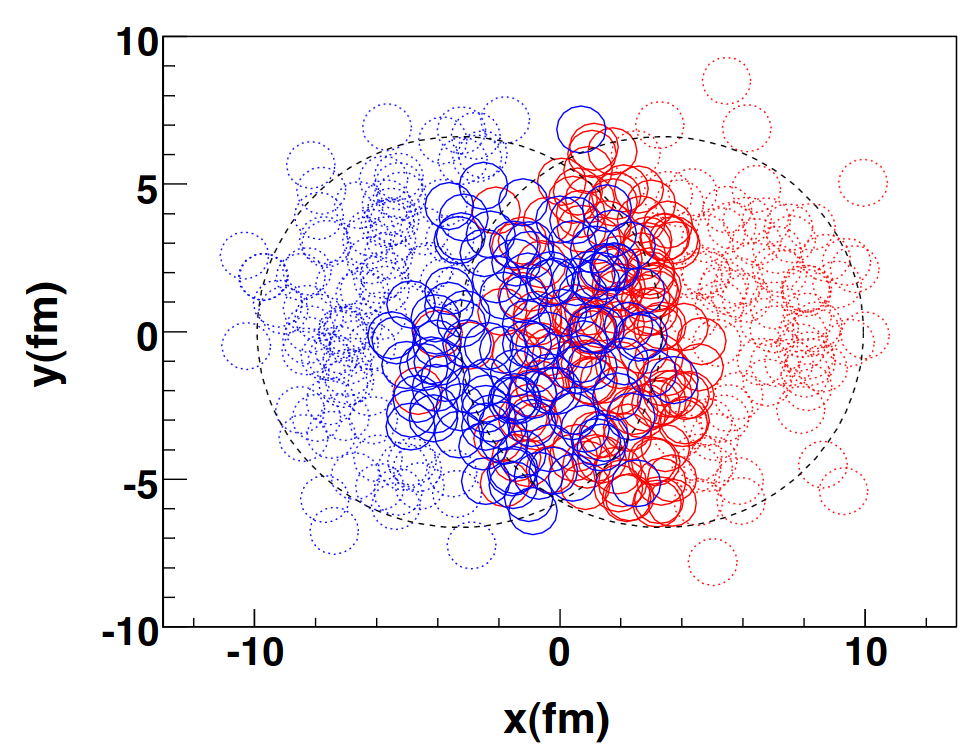
\includegraphics[width=0.7\textwidth]{glauber-collision.png}};
      \node[font=\tiny] at (1.5,-1.6) {\href{https://arxiv.org/abs/1408.2549}{arXiv:1408.2549}};
      \node[font=\tiny] at (0.2,1.8) {PbPb collision simulation};
    \end{tikzpicture}

    \

    \begin{tikzpicture}
      \node{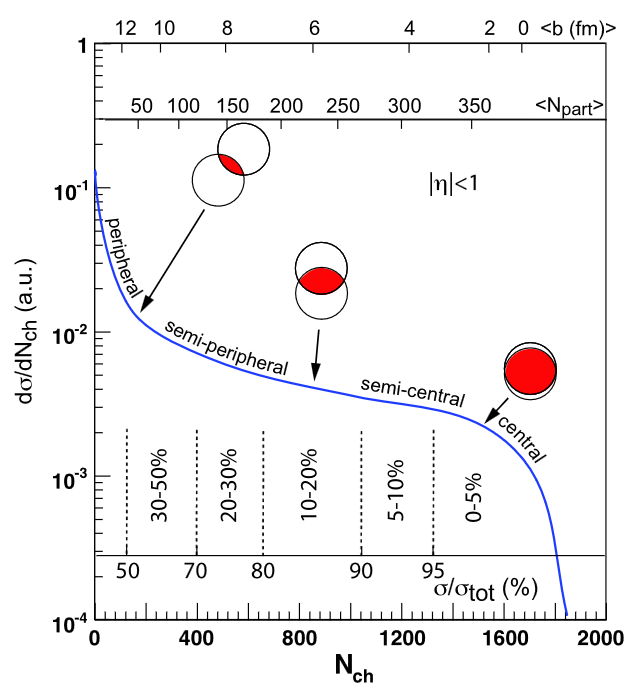
\includegraphics[width=0.65\textwidth]{centrality-nch.png}};
      \node[font=\tiny] at (1.0,-2.2) {\href{https://journals.aps.org/rmp/abstract/10.1103/RevModPhys.90.025005}{Rev. Mod. Phys. 90, 025005}};
    \end{tikzpicture}
  \end{columns}
\end{frame}
